%%%%%%%%%%%%%%%%%%%%%%%%%%%%%%%%%%%%%%%%%%%%%%%%%%%%%%%%%%%%%%%%%%%%%%%%
%                                                                      %
%     File: Thesis_Introduction.tex                                    %
%     Tex Master: Thesis.tex                                           %
%                                                                      %
%     Author: Andre C. Marta                                           %
%     Last modified : 13 May 2019                                      %
%                                                                      %
%%%%%%%%%%%%%%%%%%%%%%%%%%%%%%%%%%%%%%%%%%%%%%%%%%%%%%%%%%%%%%%%%%%%%%%%

\chapter{Introduction}
\label{chapter:introduction}

%%%%%%%%%%%%%%%%%%%%%%%%%%%%%%%%%%%%%%%%%%%%%%%%%%%%%%%%%%%%%%%%%%%%%%%%
\section{Motivation}
\label{section:motivation}

General relativity, developed by Albert Einstein, is a comprehensive theory of gravitation that fundamentally alters our understanding of the force of gravity. It portrays gravity not as a traditional force, but rather as a consequence of the curvature of spacetime caused by the presence of mass and energy. According to this theory, objects move through spacetime along paths dictated by this curvature, giving rise to the illusion of gravitational force.
\\
One intriguing prediction of general relativity is the existence of black holes, celestial objects with such immense gravitational pull that nothing, not even light, can escape their grasp. In the context of general relativity, the presence of a black hole causes spacetime to contort and deform, leading to bizarre phenomena like time dilation and the bending of light rays. To an observer located at a significant distance from a black hole, its appearance is analogous to that of a classical particle. This resemblance allows us to characterize a black hole by three primary quantities: its total mass, electrical charge, and spin. Remarkably, black holes that possess identical properties are indistinguishable, as no measurements can be made to discern their uniqueness \cite{HawMalStr16} — a concept known as the "No Hair" theorem.
\\
Understanding how different objects interact with black holes requires an exploration of the conservation laws that govern their behavior. By observing the initial and final state of an object that falls into a black hole, we can deduce a few of its properties through the lens of conservation. However, the reductionist nature of black holes poses a challenge—the wealth of information carried by stars and planets of various shapes and sizes is reduced to a mere three numbers. Consequently, a significant amount of information is lost, leading to a perplexing conundrum known as the information paradox \cite{HawMalStr16}.
\\
Expanding upon the topic, it is crucial to consider binary systems as significant sources of gravitational waves. Gravitational waves are ripples in the fabric of spacetime that propagate outward, carrying energy away from their source. Binary systems, composed of two massive objects orbiting around each other, emit gravitational waves as a result of their orbital motion. These waves can be detected and studied, providing valuable insights into the dynamics of spacetime and further confirming the predictions of general relativity.
\\
In the study of dynamical spacetime, researchers investigate the behavior of spacetime itself when subjected to the presence of matter and energy. The dynamics of spacetime can be studied by employing mathematical frameworks such as the theory of general relativity. By understanding the intricate interplay between matter, energy, and spacetime curvature, scientists gain a deeper understanding of how the fabric of the universe evolves and changes in response to different physical phenomena \cite{DaiVal02}.
\\
In summary, general relativity revolutionizes our comprehension of gravity by describing it as a consequence of spacetime curvature caused by mass and energy. Black holes, characterized by their immense gravitational pull, serve as fascinating objects that challenge our understanding of information conservation. The information paradox arises from the reduction of complex objects to a mere three numbers, leading to the potential loss of vast amounts of information. However, recent theories like soft "hair" propose avenues for exploring the consumption history of black holes and potentially resolving the information paradox. Additionally, binary systems play a crucial role in generating gravitational waves, allowing us to probe the dynamics of spacetime and deepen our understanding of the universe's fundamental nature. For general relativity, the definition of infinity is complicated as it has to surpass the ambiguity when discussing coordinate dependent notions and because there exist different types of infinities. In these report we will focus on only two types: null-infinity denoted by $\mathscr{I}$ and spatial infinity denoted by the symbol $i^0$.


%%%%%%%%%%%%%%%%%%%%%%%%%%%%%%%%%%%%%%%%%%%%%%%%%%%%%%%%%%%%%%%%%%%%%%%%
\section{Global structure of spacetimes}
\label{section:Global structure of spacetimes}

Roger Penrose brought to the field of general relativity the notion of conformal transformation, which made a significant impact in the geometric understanding of infinity. This was crucial for the development of theory of asymptotics, which arises a question of whether a smooth conformal extension which attaches a boundary - conformal boundary represents points at infinity - to the spacetime is shared by a larger class of spacetimes. This question leads to the notion of \textit{asymptotic simplicity} \cite{Val16}. In the context of asymptotic simplicity, spatial infinity (denoted as $i^0$) represents the region at an infinite distance from the central object or system under consideration. It provides a framework to analyze the properties of spacetime far away from the gravitational source. Similarly, null infinity (denoted as $\mathscr{I}$) represents the region at an infinite "time" in the future or past. It corresponds to the points reached by light rays that have traveled an infinite distance from their source. This simplicity allows for the application of mathematical techniques and tools to study the behavior of physical fields, gravitational waves, and the conservation laws in these simplified regimes.
Asymptotic simplicity is a concept in general relativity that refers to the behavior of spacetime at infinity. It characterizes the way spacetime and its geometry approach a simple and well-defined structure as we move to spatial infinity or null infinity.
\\
The geometric understanding of infinity also contributed to the development of gravitational radiation, taking a step forward in the mathematical understanding of gravitational waves. Although, customary in numerical approaches to general relativity, wave forms are computed at large radius, from first principles point of view they should be computed at null infinity $\mathscr{I}$. To do so, the Einstein field equations need to be expressed in terms of suitably rescaled fields, so one can evaluate the fields at $\mathscr{I}$. Technically this is done by a conformal transformation. In general relativity, conformal transformations are used to describe the behavior of physical systems under changes in the scale of spacetime. These transformations preserve the local structure of spacetime, but not necessarily its overall shape. The original metric, which we refer to as the physical metric, is denoted by $\tilde{g}$. We consider a transformation to an unphysical metric, $g$, which is given by 
\begin{equation}\label{eq:conftrans}
	g_{ab} = \Xi^2 \tilde{g}_{ab},
\end{equation}
$\Xi$ is a smooth function that approaches zero as the distance from the source increases. This transformation, denoted by \eqref{eq:conftrans}, preserves angles, making it appropriate to describe it as conformal. H. Friedrich introduced the \textit{conformal Einstein field
equations} (CEFE), a formulation designed that is in accordance with
the approach of R. Penrose.
\medskip

A prototypical example is the conformal extension of the Minkowski spacetime which will be discussed in the following.  One starts with the Minkowski metric line-element,
\begin{equation}\label{eq:metricMink-tr}
	d \tilde{s}^2=-d \tilde{t}^2+d \tilde{r}^2+\tilde{r}^2 d
        \Omega^2,
\end{equation}
where $(\tilde{t}, \tilde{r})$ $\in$ $(-\infty,+\infty) \times[0,+\infty)$ and $d \Omega^2$ represents the standard metric on $\mathbb{S}^2$. To get a conformal extension we need to do a coordinate transformation, corresponding to the advance and retarded  times, $\tilde{u}=\tilde{t}-\tilde{r}$ $\&$ $\tilde{v}=\tilde{t}+\tilde{r}$,  substituting equation \eqref{eq:metricMink-tr}.
\begin{equation}\label{eq:metricMink-tr1}
	d \tilde{s}^2=-d \tilde{u} d \tilde{v}+\frac{(\tilde{u}-\tilde{v})^2}{4} d \Omega^2.
\end{equation}
For the compactification, we need to introduce the following: $u = \tan U$ $\&$ $v = \tan V$, where $U$, $V$ $\in$ $(- \pi/2, \pi/2)$. Now, we are able to identify the conformal metric,
$ds$. Using \eqref{eq:metricMink-tr}, we obtain
$$d s^2=-4 d U d V+\sin ^2(V-U) d \Omega^2$$ where
$$d s^2=\Xi^2 d \tilde{s}^2$$
with $\Xi=2 \cos U \cos V$. Given the
domain of $U$ and $V$, we introduce the following, $T=V+U$ $\&$ $\psi=V-U$. The domain of $(T, \psi)$ is $(-\pi, \pi)$, with
\begin{equation}\label{eq:metricMink-cf}
	d s^2=-d T^2+d \psi^2+\sin ^2 \psi d \Omega^2,
\end{equation}
which is the metric of the Einstein static universe. The conformal boundary is given by $\psi = \pi/2$, which is the cylinder $\mathbb{S}^1 \times \mathbb{S}^2$, the Einstein Cylinder. The purpose of this thesis is  to study what happens at infinity, and in order to do that we will focus on the region where $\Xi = 0$. This condition gives us the following regions, which are presented in the following table
\begin{center}
    \begin{tabular}{ |c|c|c| }
      \hline
      Region & Name & Symbol \\
     \hline
     $\tilde{r} \rightarrow \infty \enspace \;  \text{with} \; \;\;\;\;
     |\tilde{t}| $<$ \infty$ & Spatial Infinity & $i^{0}$ \\
     \hline 
     $\tilde{t} \rightarrow \pm \infty$  \;\; with \;\; $\tilde{r}$<$\infty$
     \enspace & Future/Past Timelike Infinity & $i^{\pm}$ \\
     \hline
     $\tilde{r} \rightarrow \infty, \enspace \tilde{t} \rightarrow \infty \enspace
     \text{with} \;\; |u|$<$\infty$ &  Future Null-infinity & $\mathscr{I}^+$ \\ 
     \hline
     $\tilde{r} \rightarrow\infty, \enspace \tilde{t} \rightarrow-\infty \;\;
     \text{with} \enspace |v|$<$\infty$ & Past Null-infinity & $\mathscr{I}^-$ \\
     \hline
    \end{tabular}
    \end{center}
The visual representation of this is a Penrose Diagram, depicted in Fig.1
\begin{figure}[h]
	\centering 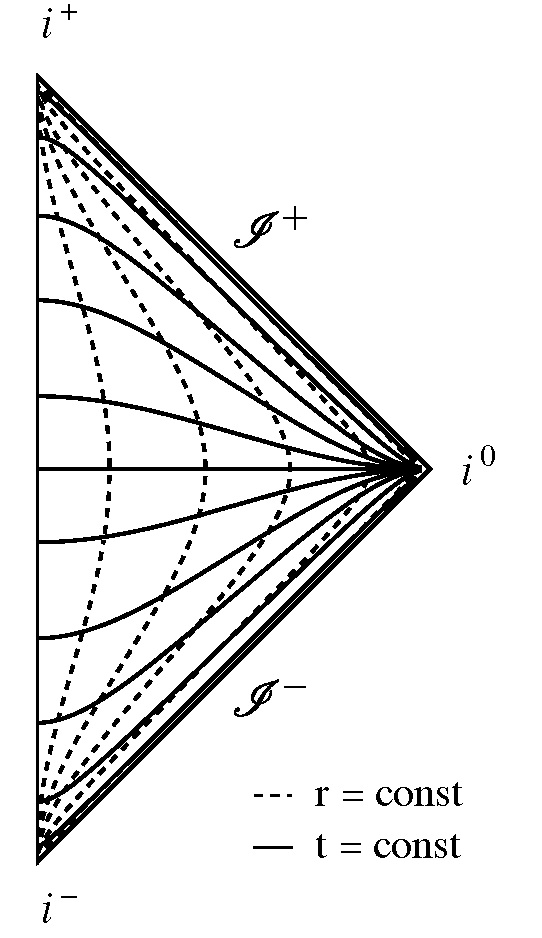
\includegraphics[width =0.3\textwidth]{Penrose diagram.pdf}
    \caption{Penrose Diagram - Representation of the standard
      compactification of the Minkowski spacetime alongside the curves of constant
      time, solid black lines, and the curves of constant r, dotted
      black lines.}
\end{figure}
\\
Additionally, H. Friedrich proposed another conformal representation of Minkowski spacetime specifically adapted for spatial infinity, which will be one used in this work. By applying the following change of coordinates $\tilde{t} = \frac{\tau}{\rho(1-\tau^{2})}$, \enspace $\tilde{\rho} = \frac{1}{\rho(1-\tau^{2})}$ we arrive at this representation. Therefore,
$$ \gamma=-d \tau^2+\frac{\left(1-\tau^2\right)}{\rho^2} d\rho^2-\frac{\tau}{\rho}(d \rho d \tau+d \tau d \rho)+d \Omega^2 $$
We are now in the position to say that the conformal factor $\Theta$ is given by,
\begin{equation}\label{eq:gamma}
	\gamma = \Theta^2 \tilde{\eta}.
\end{equation}
\begin{equation}\label{eq:conf-factor}
	\Theta = \rho(1-\tau^2).
\end{equation}
As a result of the spacetime admitting only particles that travel slower than the speed of light, which in geometric units corresponds to $\pm 1$, hence, we have  
$$ -1 \le \tau \le 1 $$ 
with $\rho$ > 0. Therefore, light travels towards infinity to the places where $\tau = \pm 1$ in the conformal extension. So, in this representation,
$$ \mathscr{I}^+ \equiv \{ \tau = 1 \}, \enspace \mathscr{I}^- \equiv \{ \tau = -1 \}$$ 
The sets where future and past null-infinities touch spatial infinity are named the critical sets and are given by,
$$ {I}^+ = \{ \tau = 1, \enspace \rho = 0\}, \enspace {I}^- = \{ \tau = -1, \enspace \rho = 0\}$$

%%%%%%%%%%%%%%%%%%%%%%%%%%%%%%%%%%%%%%%%%%%%%%%%%%%%%%%%%%%%%%%%%%%%%%%%
\section{Newman-Penrose Constants}
\label{section:Newman-Penrose Constants}
The Newman-Penrose constants, originally introduced in \cite{NewPen68}, are quantities defined on null-infinity that obey conservation laws for asymptotically flat gravitational fields. In flat spacetime, there exists an infinite number of conservation laws for each spin value. For example, in ordinary Electromagnetic (EM) theory with a spin-1 field, the total charge is conserved. In the linearized gravitational theory, which involves a spin-2 field, the total mass, linear momentum, and angular momentum are also conserved. In our case, we are interested in studying spin-0 fields, which correspond to solutions of the wave equation.
\\
The NP constants form an infinite hierarchy of conserved quantities for linear equations, including the spin-1, spin-2, and spin-0 fields. Newman and Penrose demonstrated that these constants can be expressed as the product of the square of the dipole moment and the difference between the monopole and the quadrupole moments, as shown in \cite{DaiVal02}. However, in the full non-linear gravitational theory, the conservation of mass and momentum no longer holds, leading to ten distinct conserved quantities.
\\
One intriguing question is whether the NP constants are zero for stationary spacetimes. Remarkably, for the Kerr solution and the Schwarzschild spacetime, the NP constants do vanish \cite{Bac10}, \cite{BaiZhoGonXueXiaoLau07}. The magnitude of these constants provides insights into the residual radiation present in the spacetime following a black hole collision \cite{DaiVal02}. As the NP constants retain their values along null-infinity, they offer valuable information about the behavior of black hole collisions at later times.
\\
Turning our attention to the interpretation of these charges, the NP constants are considered a set of conserved charges at null infinity \cite{NewPen68}. These charges are computed as 2-surface integrals at cuts $\mathcal{C} \approx \mathbb{S}^2$ of null infinity $\mathscr{I}$. In the linear theory, an infinite hierarchy of these conserved quantities exists, while in the non-linear theory of General Relativity, only ten quantities remain conserved \cite{NewPen68}.
\\
The interpretation of these charges is still a subject of debate [\cite{PenRin84}, \cite{DaiVal02}, \cite{Bac10}]. However, their conservation holds in general asymptotically flat spacetimes, even when the dynamics involve complex phenomena like black hole collisions \cite{DaiVal02}. Recent interest in asymptotic quantities, particularly the Bondi-Metzner-Sachs (BMS) charges, has emerged due to their connection with the concept of black hole soft hair [\cite{HawMalStr16}, \cite{HawMalStr17}, \cite{HeLyMi15}]. Understanding the relationship between conserved quantities at past and future null infinity is a crucial aspect of these discussions. However, the resolution of the singular nature of spatial infinity poses challenges in matching the conserved quantities.
\\
Therefore, the study of the Newman-Penrose constants and their conservation offers valuable insights into the dynamics of gravitational fields, particularly in black hole collisions and asymptotically flat spacetimes. These constants provide information about the residual radiation and behavior of the system at later times, shedding light on the intricate nature of spacetime and the conservation laws that govern it.
\\
The Peeling theorem, one of the most emblematic results in the classical theory of asymptotics in general relativity, has played a very important role in the development of the modern notion of gravitational radiation. It is usually formulated within the context of asymptotically simple spacetimes, as defined in Section 10.2 of \cite{Val16}.
\\
An inspection of the proof of the Peeling Theorem reveals that, in fact, it is only necessary to assume that the conformal extension is $C^{4}$.  In view of this, the question of the existence and genericity of spacetimes satisfying the peeling behavior can be rephrased in terms of the construction of asymptotically flat spacetimes with, at least, this minimum of differentiability \cite{GasVal17}. Penrose's compactification procedure, when applied to the Minkowski spacetime, yields a fully smooth conformal extension. However, for spacetimes with nonvanishing mass, such as the Schwarzschild spacetime, the conformal structure degenerates at spatial infinity. This degeneration occurs because spatial infinity can be viewed as the final point of the generators of null infinity, either in the past or future direction. As a result, it is natural to expect that the behavior of the gravitational fields near spatial infinity will somehow reflect the peeling properties of the spacetime \cite{Pen65a}.
\\
The peeling Theorem, documented in [\cite{Sac61}, \cite{BonBurMet62}, \cite{NewPen62}], represents a significant outcome in the study of asymptotic behavior in general relativity. It characterizes the decay of the Weyl tensor in the asymptotic region of the spacetime, signifying the gradual "peeling" of gravitational radiation. This theorem deepens our understanding of the intricate nature of gravitational radiation and its properties in the far-reaching regions of the spacetime.
\\
Hence, the Peeling Theorem, by decomposing the Weyl tensor into NP scalars, and the Newman-Penrose constants, by quantifying and conserving the asymptotic charges at null infinity, are interconnected concepts that deepen our understanding of the gravitational radiation and its properties in asymptotically flat spacetimes.
%%%%%%%%%%%%%%%%%%%%%%%%%%%%%%%%%%%%%%%%%%%%%%%%%%%%%%%%%%%%%%%%%%%%%%%%

\chapter{Cylinder at $i^0$}
\label{chapter:cylinder}

In Penrose's conformal approach \cite{Pen63}, the investigation of the gravitational field's decay and the asymptotic structure of spacetime is conducted not with respect to the physical spacetime $(\tilde{\mathcal{M}}, \tilde{\boldsymbol{g}})$ that satisfies the Einstein field equations $\tilde{R}_{a b}=0$. Instead, it is examined in terms of conformally related spacetime $(\mathcal{M}, \boldsymbol{g})$, referred to as the unphysical spacetime, where $\boldsymbol{g}=\Omega^2 \tilde{\boldsymbol{g}}$. The conformal factor $\Omega$ plays a crucial role as a boundary defining function. Specifically, it defines the set of points $\mathscr{I}$ in the unphysical manifold where $\Omega = 0$ while ensuring that $d\Omega \neq 0$.
\\
Within the conformal structure of asymptotically flat spacetimes, a distinguished point is spatial infinity $i^0$, characterized by $\Omega = 0$ and $d\Omega = 0$. Extensive discussions on the conformal approach and the conformal Einstein field equations can be found in [\cite{Val16}, \cite{Fra04}, \cite{Fri02}]. This comprehensive exploration delves into the nuances of the conformal methodology and its implications for understanding the asymptotic behavior and structure of spacetime.
%%%%%%%%%%%%%%%%%%%%%%%%%%%%%%%%%%%%%%%%%%%%%%%%%%%%%%%%%%%%%%%%%%%%%%%%

\section{The $i^0$ - cylinder representation in Minkowski  spacetime}
\label{the $i^0$ cylinder}

Consider the spherical polar coordinates denoted by $(\tilde{t}, \tilde{\rho}, \vartheta^A)$ with $A = 1, 2$, where $\vartheta^A$ represents a set of coordinates on $\mathbb{S}^2$. In this coordinate system, the metric of \textit{physical} Minkowski spacetime is given by $\tilde{\eta}$
\begin{equation}\label{eq:physicalMikmetric}
\tilde{\boldsymbol{\eta}}=-\mathbf{d} \tilde{t} \otimes \mathbf{d} \tilde{t}+\mathbf{d} \tilde{\rho} \otimes \mathbf{d} \tilde{\rho}+\tilde{\rho}^2 \boldsymbol{\sigma}.
\end{equation}
In the specific range, $\tilde{t} \in (-\infty, \infty)$, $\tilde{\rho} \in [0, \infty)$, where $\sigma$ denotes the standard metric on $\mathbb{S}^2$, we introduce \textit{unphysical} spherical polar coordinates $(t, \rho, \vartheta^A)$ as an intermediate step towards obtaining the desired conformal representation
\begin{equation}\label{eq:unphysicalCoords}
t=\frac{\tilde{t}}{\tilde{\rho}^2-\tilde{t}^2}, \quad \rho=\frac{\tilde{\rho}}{\tilde{\rho}^2-\tilde{t}^2}.
\end{equation}
By expressing the physical Minkowski metric $\tilde{\eta}$ in terms of the unphysical spherical polar coordinates $(t, \rho, \vartheta^A)$, one can easily recognize the \textit{inversion} conformal representation of the Minkowski spacetime $(\mathbb{R}^4, \eta)$, where:
\begin{equation}\label{eq:metricRelation}
  \boldsymbol{\eta} = \Xi^2 \boldsymbol{\tilde{\eta}},
\end{equation}
with
\begin{equation}\label{eq:Unphysicalspacetimemetric}
  \boldsymbol{\eta}=-\mathbf{d} t \otimes \mathbf{d} t+\mathbf{d} \rho \otimes \mathbf{d} \rho+\rho^2 \boldsymbol{\sigma}, \quad \Xi=\rho^2-t^2
\end{equation}
In this conformal representation, where $t \in (-\infty, \infty)$, $\rho \in [0, \infty)$, the spatial infinity and the origin undergo an interchange. This implies that $i^0$ is represented by the point $(t = 0, \rho = 0)$ in $(\mathbb{R}^4, \eta)$. Introducing the coordinates $(\tau, \rho, \vartheta^A)$, where $t = \rho \tau$, and considering the conformal metric $\boldsymbol{g} = \rho^{-2} \boldsymbol{\eta}$, we obtain:
\begin{equation}\label{eq:unphysicalmetricMink}
\boldsymbol{g}=-\mathbf{d} \tau \otimes \mathbf{d} \tau+\frac{\left(1-\tau^2\right)}{\rho^2} \mathbf{d} \rho \otimes \mathbf{d} \rho-\frac{\tau}{\rho} \mathbf{d} \rho \otimes \mathbf{d} \tau-\frac{\tau}{\rho} \mathbf{d} \tau \otimes \mathbf{d} \rho+\boldsymbol{\sigma}
\end{equation}
In this context the \textit{unphyical metric $\boldsymbol{g}$} is related to the physical metric through the following relationship:
\begin{equation}\label{eq:gandtheta}
\boldsymbol{g}=\Theta^2 \tilde{\boldsymbol{\eta}}, \quad \text { where } \quad \Theta:=\frac{\Xi}{\rho}=\rho\left(1-\tau^2\right).
\end{equation}
The unphysical metric $\boldsymbol{g}$, also known as the $i^0$ - cylinder metric, is associated with the coordinates $(\tau, \rho, \vartheta^A)$, which are commonly referred to as the $F$ - coordinates system.
The F-coordinate system can be related to the physical polar coordinates through the following relation:
\begin{align}\label{Ftophys}
\tau = \frac{\tilde{t}}{\tilde{\rho}}, \qquad \rho = \frac{\tilde{\rho}}{\tilde{\rho}^2-\tilde{t}^2},
\end{align}
the inverse transformation is given by
\begin{align}\label{phytoF}
\tilde{t} = \frac{\tau}{\rho (1-\tau^2)}, \qquad \tilde{\rho}=\frac{1}{\rho (1-\tau^2)}.
\end{align}
Upon unwrapping the definitions, the conformal factor $\Theta$ in $F$-coordinatesystem and physical coordinates can be expressed as follows:
\begin{align}
\Theta = \rho (1-\tau^2) = \frac{1}{\tilde{\rho}}
\end{align}
The inverse transformation in \eqref{phytoF} can be written as
\begin{align}
\tilde{t}=\frac{\tau}{\Theta}, \qquad \tilde{\rho}= \frac{1}{\Theta}.
\end{align}
Furthermore, it is worth noting that the physical retarded and advanced times, denoted as $\tilde{u}:=\tilde{t}- \tilde{\rho}$ and 
\\$ \tilde{v}:= \tilde{t}+ \tilde{\rho}$, respectively, can be related to the unphysical advanced and retarded times as follows:
\begin{align}\label{eq:UnphysPhysAdvRet}
v:=t-\rho=-\rho(1-\tau)=\tilde{v}^{-1}, \qquad u:=t+\rho=\rho(1+\tau)=-\tilde{u}^{-1}.
\end{align}
In this conformal representation of the Minkowski spacetime, future and past null infinity can be identified at the following locations:
\begin{align}
\mathscr{I}^{+} \equiv \{ p \in \mathcal{M} \; \rvert\; \tau(p) =1\}, \qquad \mathscr{I}^{-} \equiv \{ p \in \mathcal{M} \; \rvert \;\tau(p) =-1\}.
\end{align}
The term $i^0$ - cylinder derives from the observation that spatial infinity is mapped to an extended set $I \approx \mathbb{R}\times \mathbb{S}^2$.
\begin{align*}
I \equiv \{ p \in \mathcal{M} \; \rvert \;\; |\tau(p)|<1, \;\rho(p)=0\}, \qquad I^{0} \equiv \{ p \in \mathcal{M}\; \rvert \;\tau(p)=0, \; \rho(p)=0\},
\end{align*}
where the regions spatial and null infinity meet were already defined in section 1.2.